% =====================================================================
\chapter{Notação Ω: o piso}\label{cap:06}
\naaula{24, 26 e 27}

Se $O$ é um teto, $\Omega$ (lê-se \enquote{ômega grande}) é um \textbf{piso}: escrever
$f(n) = \Omega(g(n))$ significa que \textbf{$f$ cresce pelo menos tão rápido quanto $g$}.

\section{A definição}

\begin{center}
\colorbox{edtealclaro}{\parbox{0.92\textwidth}{\centering\large
$f(n) = \Omega(g(n))$ \ se existem constantes $c > 0$ e $n_0 \ge 1$ tais que\\[0.3em]
$f(n) \ge c \cdot g(n)$ \ para todo $n \ge n_0$.}}
\end{center}

É a mesma definição do $O$, com a desigualdade virada: agora $f$ fica \textbf{acima} de
$c \cdot g$ a partir de $n_0$.

\begin{figure}[!htb]
  \centering
  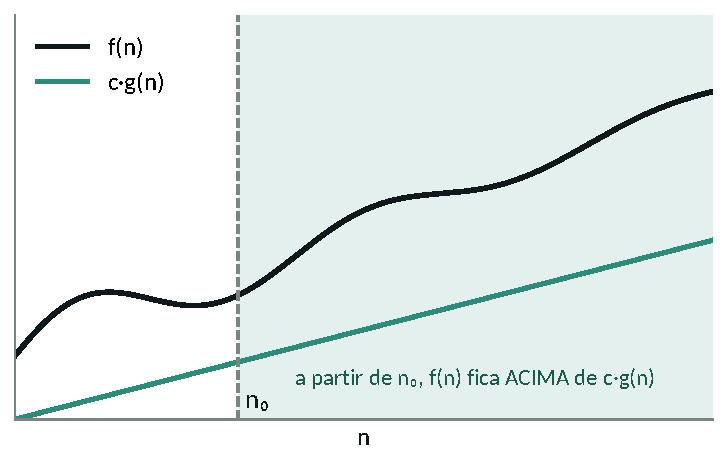
\includegraphics[width=0.72\textwidth]{figuras/f06_definicao_Omega.pdf}
  \caption{A partir de $n_0$, $f$ nunca desce abaixo do piso $c \cdot g(n)$.}
\end{figure}

\section{Exemplos}

\textbf{$3n + 4 = \Omega(n)$.} Com $c = 3$: $3n + 4 \ge 3n$ vale para todo $n \ge 1$ (o $+4$ só
ajuda). Então $c = 3$ e $n_0 = 1$. (É a reta $3n$ da figura~\ref{fig:exemplo3n4}.)

\textbf{$\dfrac{n^2}{2} - 3n = \Omega(n^2)$.} Aqui há um termo \emph{subtraindo}, então precisamos
de um pouco mais de cuidado. Vamos tentar $c = \dfrac{1}{4}$:
\[
\frac{n^2}{2} - 3n \ge \frac{n^2}{4}
\;\Longleftrightarrow\; \frac{n^2}{4} \ge 3n
\;\Longleftrightarrow\; n \ge 12.
\]
Então $c = \dfrac{1}{4}$ e $n_0 = 12$ funcionam. A ideia: \enquote{gastamos} metade do termo
dominante para cobrir o termo negativo, que é menor.

\section{Ω também descreve problemas}

A notação $\Omega$ tem um uso muito poderoso: dizer que um \textbf{problema} exige, no mínimo,
certo trabalho, qualquer que seja o algoritmo.

\begin{intuicao}
Achar o maior valor de uma lista \textbf{não ordenada} com $n$ elementos exige olhar todos os
$n$. Por quê? Se algum algoritmo deixasse de olhar um único elemento, esse elemento poderia ser
justamente o maior, e o algoritmo erraria. Então todo algoritmo correto para esse problema faz
pelo menos $n$ leituras: o problema é $\Omega(n)$. Nenhuma ideia genial, em nenhuma linguagem,
consegue fazer melhor.
\end{intuicao}

\section{Como mostrar que algo NÃO é Ω}

Será que $n = \Omega(n^2)$? Precisaríamos de $n \ge c \cdot n^2$, ou seja, $1 \ge c \cdot n$,
ou ainda $n \le \dfrac{1}{c}$. Como $n$ cresce sem parar, isso falha para $n$ grande. Então
$n$ \textbf{não} é $\Omega(n^2)$: uma função linear não cresce tão rápido quanto uma quadrática.

\begin{exrapido}
(a) Mostre que $5n - 20 = \Omega(n)$. (b) $n = \Omega(n^2)$? (c) $n^2 = \Omega(n)$?
\end{exrapido}

\begin{respostas}
  \resp{6.1} (a) Com $c = 1$: $5n - 20 \ge n \Longleftrightarrow 4n \ge 20 \Longleftrightarrow n \ge 5$.
  Então $c = 1$ e $n_0 = 5$. (b) Não (seção 6.4). (c) Sim: $n^2 \ge 1 \cdot n$ para todo $n \ge 1$.
  Um piso baixo é sempre verdadeiro, mas, como o teto alto do $O$, é pouco informativo.
\end{respostas}
